% !Mode::"TeX:UTF-8"
\documentclass[a4paper,12pt]{article}
\usepackage{ctex} %中文支持
\usepackage{amsmath} %数学公式 符号
\usepackage{amsthm} %定理格式
%\usepackage{DefaultTheormStyle} %这个如果要用的话 就手动打进来
\usepackage{lastpage}
\usepackage{makecell} %表格线加粗 \Xhline{1.2pt}
\usepackage{boldline} %长表格表格线加粗
\usepackage{multirow} %合并单元格
\usepackage{array}
\usepackage{longtable} %长表格
\usepackage[dvipsnames]{xcolor} %颜色声明
\usepackage{varioref} %For Cross References
\renewcommand{\reftextbefore}
    {on the \reftextvario{preceding page}{page before}}
\renewcommand{\reftextafter}{(见下页)}
%\renewcommand{\reftextfacebefore}
%    {on the \reftextvario{facing}{preceding} page}
%\renewcommand{\reftextfaceafter}
%    {on the \reftextvario{facing}{next}{page}}
\renewcommand{\reftextfaraway}[1]{在第\pageref{#1}页}
\usepackage{caption} %题注
\captionsetup{margin    =   6pt,
              font      =   footnotesize,
              labelfont =   bf}
\usepackage{fancyhdr} %脚注
\setlength{\headheight}{15pt}
\lhead{Team tsp}
\rhead{Page \thepage\ of \pageref{LastPage}}
\usepackage[square, numbers, sort&compress]{natbib} %引用
\renewcommand{\bibsection}{} %不显示"Reference"
\usepackage{hyperref}
\hypersetup{linktoc             =   all,
            colorlinks          =   true,
            linkcolor           =   Black,
           %anchorcolor         =   Black,
            citecolor           =   NavyBlue,
           %filecolor           =   Cyan,
           %menucolor           =   Red,
           %runcolor            =   filecolor,
            urlcolor            =   magenta,
            pdfinfo             =   {
                Title           =   {数学建模论文大作业模板},
                Author          =   {陈旭阳},
                Subject         =   {数学建模 论文模板}},
            bookmarksnumbered   =   true,
            pdfstartview        =   FitH,
            pdfpagelayout       =   OneColumn}
\renewcommand{\tablename}{表}
\renewcommand{\figurename}{图}
\renewcommand{\contentsname}{目录}
\renewcommand{\abstractname}{摘要}
\usepackage{graphicx}
\graphicspath{{Figures/}} %图像文件目录
\usepackage[section]{placeins} % 使图像不会显示在别的部分 若过于严格则换成[below]
%\usepackage{fontspec} % 字体
\theoremstyle{definition}
\newtheorem{dfn}{定义}[subsection]
\newtheoremstyle{Note}% name
    {3pt}% Space above
    {3pt}% Space below
    {\itshape}% Body font
    {}% Indent amount
    {\itshape}% Theorem head font
    {:}% Punctuation after theorem head
    {.5em}% Space after theorem head
    {}% Theorem head spec (can be left empty, meaning `normal')
\theoremstyle{Note}
\newtheorem{note}{注}[subsection]
\usepackage{titlesec} %Section标题格式
\usepackage{SUBSubsubsection}
\usepackage{authblk} %作者
\usepackage{stackrel} %上下写
\usepackage{enumitem}
\usepackage{listings} %排版程序语言

%===============TITLE===============
\title{演绎法数独生成和基于深度优先搜索的Kakuro求解分级模型}
\author{1752161 姚鸿增, 1753309 毕晓栋, 1753763 陈旭阳}
\affil{Team tsp}
\date{2018年03月31日}

\begin{document}
    \pagestyle{empty}
    \pagenumbering{roman}
    \maketitle
    \newpage
    \tableofcontents
    \newpage

%===============ABSTRACT===============
    % !Mode::"TeX:UTF-8"
\begin{abstract}
    本文主要建立了Kakuro求解算法模型,
    Kakuro难度评估模型, 蜂巢数独求解模型,
    并且还给出了生成不同难度和具有唯一解的Kakuro的方法.
    
    在求解Kakuro数独和求解蜂巢数独的模型中,
    本文使用深度优先搜索的算法, 
    采用了回溯的思想,
    并采用人们所常用的几个数独技巧作为剪枝方法, 其中包括了可行性剪枝, 最优化剪枝和归谬法剪枝,
    实现了两种不同数独的快速求解.
    在蜂巢数独求解模型中, 本文将一整行当作一个状态, 从而只用较少的递归次数就能实现数独的求解.
    在建立难度评估系统模型中, 本文基于深度优先搜索树的性质,
    搜索树上根节点到目标节点的唯一路径的分支总数来刻画数独的难度, 得出了难度评估公式,
    并给出了分级标准, 实现了对Kakuro数独不同难度的划分.
    对于Kakuro的生成的方法, 本文使用演绎法, 先确定数独中黑格子的位置,
    再一步步地添加约束条件, 在保证数独的唯一解的原则下, 由局部到整体地生成数独.
    
    本文的模型能够在极短的时间内对两种数独进行求解, 在所有搜集到的两种数独之中,
    Kakuro都能在1s以内计算出结果,
    蜂巢数独能在0.1s以内完成求解.
    本文建立的难度评估系统, 在实例分析中, 能够对不同难度的Kakuro数独实现较为准确的分级,
    且具有稳定性, 可以不受搜索的随机性的影响.
    本文建立的数独生成模型能够生成不同难度具有唯一解的数独, 并且难度可以在生成之前指定.
\end{abstract}


%===============KEYWORDS===============
    \small{\textbf{关键词}:
        深度优先搜索, 回溯法, 可行性剪枝, 最优化剪枝, 演绎法, 唯一解生成, Kakuro, 蜂巢数独.}

    \thispagestyle{empty}
    \newpage

%===============BODY===============
    \pagestyle{fancy}
    \pagenumbering{arabic}
    % !Mode::"TeX:UTF-8"

%===============INTRODUCTION===============
\section{背景介绍}
    \subsection{问题重述}
        数独(Sudoku)是一种运用纸笔进行验算的智力游戏\citep{Baidu_Sudoku},
        由十八世纪著名数学家欧拉所发明,
        旨在通过数字的推理来锻炼人们的思维, 容易上手, 易于沉迷.
        而Kakuro作为普通数独的推广, 比Sudoku更加难玩,
        除了涉及逻辑推理, 更要大家计算加数\citep{Baidu_Kakuro}.
        它与Sudoku玩法相近, 但趣味更丰富, 挑战性更大.

        Kakuro的主要规则有:
        \begin{itemize}
            \item 在空格中填入数字1-9, 数字0不能出现.
            \item 带斜线的方格, 斜线上方的数字等于该方格右面对应的一组水平空格的数字之和;
                    斜线下方的数字, 等于该方格下面对应一组垂直空格里的数字之和.
            \item 同一个数字在每组水平(垂直)的空格里只能出现一次.
        \end{itemize}

        在本文中,我们要完成以下任务:
        \begin{itemize}
            \item 讨论并找出一种求解Kakuro数独的算法模型, 并且对算法的复杂度进行讨论.
            \item 给出一种Kakuro级别划分系统, 给出具体的划分方式和划分公式,
                    并且对该级别划分系统进行实例检验.
            \item 给出一种生成不同难度且具有唯一解的数独的方法.
            \item 利用Kakuro数独的求解模型, 对蜂巢数独进行求解并进行实例检验.
        \end{itemize}

    \subsection{解题途径}
        写程序解Kakuro之前, 我们先分析了人解Kakuro时可能用到的技巧.
        \begin{enumerate}
            \item \textbf{数集缩小}: 通过所给的和来确定每行每列的所填情况和候选数集,
                    初步将原先1—9的范围缩小.\label{Skill1}
            \item \textbf{交叉影线}: 查找交叉的一行一列, 比较它们的候选数集,
                    则交叉的白格填入的数字一定是它们候选数集交集的元素.
                    如果元素唯一, 则交叉白格的数字确定.
                    我们首先要找的便是交集唯一的行与列, 进而确定交叉的白格.\label{Skill2}
            \item \textbf{组合参考}: 在使用交叉影线的技巧确定完所有可确定的白格后,
                    更新每行每列的候选数集(一般可将能填情况缩小为1-2种), 之后进行深一步的考虑.
                    对于每行(列), 考虑它候选数集中的最大最小数, 并与交叉的列(行)进行比对,
                    可缩小交叉白格的候选数集或限制所填情况, 进而确定该行唯一的填写情况(此时序列不确定,
                    但数的集合确定).\label{Skill3}
            \item \textbf{假设推理}: 当白格中填写的数字只有2种可能时,
                    可假设填写其中的一个, 再结合其他行列进行推理判断, 如该数字是否与其他行列的数字重复,
                    有没有导致其他行列无法达到所给之和等, 进而确定白格中的数字.\label{Skill4}
        \end{enumerate}

        在求解Kakuro过程中, 我们使用深度优先搜索算法,
        并采用了上述几种人们常用的技巧作为剪枝方法.
        在求解蜂巢数独的过程中, 我们同样在算法中体现了人们经常使用的技巧.
        在建立难度评估系统模型中, 我们基于程序采用技巧时的不确定性以及采用归谬法的次数,
        来计算难度评估公式.
        对于Kakuro的生成的方法, 本文使用演绎法, 运用上述的解题技巧进行逆向推理,
        从而生成给定难度的具有唯一解的数独.

%===============ASSUMPTION===============
\section{模型假设} %分析
    \begin{itemize}
        \item 本文中讨论的Kakuro都是以$8\times10$作为大小, 且最上一行和最左一列均为不能填数的格子.
        \item 本文中的Kakuro没有只有一个元素的一组数字.
        \item 网上搜寻的Kakuro符合要求.
    \end{itemize}
%===============NOTATIONS===============
\section{符号介绍}
    \begin{center}
        \begin{tabular}{cc}
            \Xhline{1.2pt}
            符号              &   意义\\
            \hline
            $\log(x)$         &   $x$的自然对数\\
            $n$-in-$m$        &   和为$n$, 组内数字个数为$m$的一种约束\\
            $S(x,y)$          &   见定义\ref{dfnSet}\\
            $S_{r}(x,y)$      &   见定义\ref{dfnRow}\\
            $S_{c}(x,y)$      &   见定义\ref{dfnRow}\\
            $O$               &   算法时间复杂度上限\\
            $W$               &   深度优先搜索树的路径复杂度\\
         %  $s_{1}$           &   深度优先搜索树初始节点到目标节点的路径上出度为一的节点的数量\\
         %  $s_{2}$           &   深度优先搜索树初始节点到目标节点的路径上出度为二的节点的数量\\
         %  $s_{3}$           &   深度优先搜索树初始节点到目标节点的路径上出度为三的节点的数量\\
            $R$               &   难度函数\\
            {$P(a_{1},a_{2},\dotsc,a_{n})$}   &
                $\{(a_{b_{1}},a_{b_{2}},\dotsc,a_{b_{n}})\mid\bigcup\limits_{i=1}^n{b_{i}}=\{1,2,\dotsc,n\}\}$\\
                              &   $a_{1},a_{2},\dotsc,a_{n}$所有排列构成的集合\\
            白格子            &   允许填入数字的格子\\
            黑格子            &   不能填入数字的格子\\
            \Xhline{1.2pt}
        \end{tabular}
    \end{center}

%===============MODELING===============
\section{模型的建立与求解}
    \subsection{Kakuro求解算法}\label{sec1}
        \subsubsection{概述}
            首先, 看到问题我们有两种思路,
            一种是采用深度优先搜索(Depth-first search),
            另一种是采用广度优先搜索(Breadth-first search).
            如果采用广度优先搜索, 能够避免程序陷入死角, 时间复杂度低, 能更快的实现搜索, 但是空间复杂度高.
            而深度优先搜索算法则有较小的空间复杂度.
            经过权衡比较, 因为广度优先搜索算法的空间复杂度预估过高, 我们采用了深度优先搜索算法的算法.
            可是如果是裸的深度优先搜索算法, 时间复杂度高达$\Theta(n!)$, 这绝对不是一个能够承受的复杂度,
            因此, 我们就要考虑利用人们做Kakuro的技巧进行剪枝.
        \subsubsection{基本定义}
            \begin{dfn}
                一个白格子的\textbf{策略}指经过一定的逻辑推理之后, 可能填入该格子的数.
            \end{dfn}
            \begin{dfn}\label{dfnSet}
                对于一个坐标在$(x,y)$的白格子, 其策略的集合为该白格子的\textbf{策略集},
                记为$S(x,y)$, 不引起混淆的情况下, 可简记为$S$.
            \end{dfn}
            \begin{dfn}\label{dfnRow}
                对于一个坐标在$(x,y)$的白格子, 它被同一行(列)的黑格子约束,
                则将仅受到此约束时可能填入的数的集合,
                称为该白格子的\textbf{行(列)约束策略集}, 记为$S_{r}(x,y)$ $(S_{c}(x,y))$,
                不引起混淆的情况下, 可简记为$S_{r}$ $(S_{c})$.
            \end{dfn}
            为了减小白格子策略集中元素的个数, 从而减小解出白格子的时间复杂度, 我们规定了如下剪枝技巧.

        \subsubsection{交集剪枝法}
            根据\vpageref*{Skill2}的技巧\ref{Skill2},
            人解Kakuro的时候会取行约束策略集和列约束策略集的交集,
            以减少白格子策略集的元素.

            \label{dfnCap}\textbf{交集剪枝}:
                设白格子$(x,y)$分别受到两个黑格子的行约束和列约束, 则\[S(x,y)=S_{r} \cap S_{c}.\]
            \paragraph{交集剪枝的例子}
                \begin{figure}[htb]
                    \centering
                    \includegraphics[scale = 0.5]{example1-1.bmp}
                    \caption[例1-1]{交集剪枝的例子-题目}\label{exm1-1}
                \end{figure}
                如图\ref{exm1-1}, 求问号处白格子的策略集。因为19-in-3可分为
                \begin{equation*}
                    \begin{split}
                        19\ & = 2+8+9\\
                            & = 3+7+9\\
                            & = 4+6+9\\
                            & = 4+7+8\\
                            & = 5+6+8,
                    \end{split}
                \end{equation*}
                并且4-in-2可分为
                \[4 = 1 + 3,\]
                因此\[S_{r}=\{2,3,4,5,6,7,8,9\},\] \[S_{c}=\{1,3\}.\]
                根据定义\ref{dfnCap}, 可知$S=S_{r} \cap S_{c}=\{3\},$
                即问号处白格子只能填入3.
                \begin{figure}[htb]
                    \centering
                    \includegraphics[scale = 0.5]{example1-2.bmp}
                    \caption[例1-2]{交集剪枝的例子-答案}\label{exm1-2}
                \end{figure}

            通过这个例子, 我们可以看出, 运用交集剪枝可以使每个白格子策略集元素个数大大减少, 甚至能够唯一确定,
            这将为深度优先搜索的可行性奠定基础.
            并且任一$n$-in-$m$情况的行(列)约束策略集是我们能够在程序运行之前通过回溯算法预处理出的,
            且时间复杂度较低.

        \subsubsection{重复性判定剪枝}
            \label{dfnDup}\textbf{重复性判定剪枝}:
                根据在同一个约束下数字不能重复的规则, 通过判断是否重复, 来再次减少策略集元素的个数.
            \paragraph{重复性判定剪枝的例子}
                \begin{figure}[htb]
                    \centering
                    \includegraphics[scale = 0.5]{example2.bmp}
                    \caption[例2]{重复性判定剪枝的例子}\label{exm2}
                \end{figure}
                如上图, 根据交集剪枝, 我们已经知道了问号处白格子的策略集$S=\{1,3\}$,
                但因为同样的行约束中已经填入了1, 因此$S=\{1,3\}-\{1\}=\{3\}$, 即问号中只能填入3.
                程序中, 我们建立了一个bool类型的数组, 来判断在$(x,y)$处的白格子填入$n$是否会造成重复.

            通过重复性判定剪枝, 我们可以再次减少策略集元素的个数. 此方法是一个非常有效的剪枝.

        \subsubsection{最优化剪枝}
            在一个约束条件下, 有若干组可能的加数组合.
            如果当约束内有一个或多个数被确定, 有可能会导致某种组合不再可能, 从而可能导致有的数不再可能被填入,
            因此我们可以将这些数(不仅仅是已经确定被填入的数)从策略集中删去.
            在具体的算法实现中, 我们定义了如下方法.
            \label{dfnOpt}\textbf{最优化剪枝}:
                参见\vpageref*{Skill3}的\ref{Skill3},
                当我们在某个白格子的策略集中挑选数时, 如果我们所选的数,
                使得同一个约束下的别的白格子即使取最优值, 仍然不能满足该约束,
                那么我们就舍去这种方案.
            \paragraph{最优化剪枝的例子}
                \begin{figure}[htb]
                    \centering
                    \includegraphics[scale = 0.5]{example3.bmp}
                    \caption[例3]{最优化剪枝的例子}\label{exm3}
                \end{figure}
                我们知道20-in-3可分为
                \begin{equation*}
                    \begin{split}
                        20\ & = 3+8+9\\
                            & = 4+7+9\\
                            & = 5+7+8,
                    \end{split}
                \end{equation*}
                因为3已经填入, 所以问号处白格子的策略集$S=\{4,5,7,8,9\}$.
                如果在问号处填入4, 5或7, 即使空白的白格子中填入9, 都有这三个数的和小于20, 无法满足约束条件,
                因此问号处白格子的策略集$S=\{4,5,7,8,9\}-\{4,5,7\}=\{8,9\}$.
                策略集中的元素进一步减少.

        \subsubsection{归谬法剪枝}
            根据\vpageref*{Skill4}的技巧\ref{Skill4},
            如果人无法或难以直接推理出结果, 会采用归谬法.
            因此在算法中我们也体现了这一点.
            \label{dfnCtd}\textbf{归谬法剪枝}:
                当一个白格子的策略集中有不止一个元素, 我们假设填入一个数,
                如果经过之后的逻辑推理得出矛盾, 那个可以从策略集中删去这个数.
            \paragraph{归谬法剪枝的例子}
                \begin{figure}[htb]
                    \centering
                    \includegraphics[scale = 0.6]{example4.bmp}
                    \caption[例4]{归谬法剪枝的例子}\label{exm4}
                \end{figure}
                这是题目给出样例的局部, 我们从中截取了此例所需的部分, 并定义了坐标.
                当我们试图推理问号(2,2)处的值时, 易知$S(2,2)=\{1,2\}.$
                如果我们填入1, 则在问号右边的两个白格子处,
                只能一个填入7, 一个填入9, 即$S(3,2)=S(4,2)=\{7,9\}.$
                但是(3,2)的格子受到了(3,6)黑格子的16-in-5的列约束, 而16-in-5仅可分为\[16=1+2+3+4+6,\]
                即$S_{c}(3,2)=\{1,2,3,4,6\}.$
                此时发现$S(3,2)\cap S_{c}(3,2)=\emptyset,$
                推出谬误.

            归谬法剪枝是一种十分有效, 对解题关键且难度较大的技巧.\label{xplCtd}
            因此, 我们将把程序解Kakuro数独时使用归谬法剪枝的次数作为难度分级的重要依据之一.

        \subsubsection{贪心算法}
            为了加快搜索速度, 我们采用贪心的思想进行搜索.
            \label{dfnGrd}\textbf{贪心算法}是每次选取格子的时候选取策略集内元素最少的格子进行搜索.
            这是一种能够保证正确且有效的贪心算法, 而且符合人类解数独的思维,
            这个贪心将为我们用程序来衡量数独难度中关键所在.

        \subsubsection{算法复杂度}
            因为使用了大量的剪枝, 只能分析出算法的时间复杂度上限为$O(n!),$
            不过事实上, 实际时间复杂度远小于时间复杂度上限.
            以题目中样例为例, 见\vpageref*{resKak}的程序运行结果截图,
            程序共递归次数仅1544次, 所耗时间0.1秒之内.

            经过大量的测试, 能够搜集到的数独中, 此程序都能在几千次搜索内完成,
            运行时间均在0.1秒以内, 能实现数独的快速解决.
            可见, 本算法是一种高效的解决方案.
            程序由c++语言编写, 附\vpageref*{prgKak}中.

    \subsection{Kakuro难度划分}
        \subsubsection{对运算量的思考}
            因为程序是按照人类的思维进行编写的, 所以其运算量能够在一定程度上反应数独的难度.
            但是, 通过测试我们发现, 运算量有很大的随机性.
            比如说同一个数独, 从1到9枚举和从9到1,运算量差距很大.
            对于题目给出的样例, 如果逆序枚举策略,
            运算只需要91次, 远远小于正序枚举策略的1544次.

            可见, 通过运算量来评估数组难度是不合理的甚至是荒谬的.
            因此, 我们需要建立一种新型的评测机制.

        \subsubsection{对空格数和约束数量的思考}
            经过实践发现, 即使空格数目相同, 约束数目相同, 且布局相似的数独,
            难度仍有天壤之别. 因此空格数目和约束数目无法作为分级的依据.

        \subsubsection{基于深度优先搜索树和归谬法次数的难度评估系统}
            \subsubsubsection{深度优先搜索树的路径复杂度}
                \begin{figure}[htb]
                    \centering
                    \includegraphics[scale = 0.75]{bfstree.bmp}
                    \caption[bfs搜索树]{深度优先搜索树}\label{bfsTre}
                \end{figure}
                图\vref*{bfsTre}是深度优先搜索树, 每个节点表示一个数独的状态,
                节点的分支数表示某次策略所选的格子的策略集的元素数目.
                \begin{dfn}\label{dfnCpl}
                    \textbf{路径复杂度}:
                    \[W=1^{s_{1}}\times2^{s_{2}}\times3^{s_{3}},\]
                    其中
                    \begin{itemize}
                        \item $s_{1}$: 深度优先搜索树初始节点到目标节点的路径上出度为一的节点的数量
                        \item $s_{2}$: 深度优先搜索树初始节点到目标节点的路径上出度为二的节点的数量
                        \item $s_{3}$: 深度优先搜索树初始节点到目标节点的路径上出度为三的节点的数量
                    \end{itemize}
                \end{dfn}
                图\ref{bfsTre}中, 路径上的点已经用绿色标识,
                其中$s1=2, s2=1, s3=1,$ 则$W=2*3=6.$

                可见, $W$反应了从初始状态到目标状态中, 所选择策略的不确定性的评估.
                当使用前文常用的三个剪枝后, 如果策略还不能唯一确定, 就说明产生了分歧,
                而$W$正是一个评测这种分歧多少的量.
                注意, $W$和总运算量有所不同,
                总运算量会受到枚举顺序的影响(正序枚举策略集和倒序枚举策略集的元素).
                但是$W$却不受到此影响, 这是因为树上初始节点和目标节点的路径是唯一的,
                因此$s_{1}, s_{2}, s_{3}$不受到枚举顺序的影响, $W$也是唯一确定的.
            \subsubsubsection{归谬法的次数}
                为了叙述方便, 记程序中归谬法剪枝使用的次数为$c$.

                \vpageref*[上面][]{xplCtd}已经说过归谬法是一种难度较大的剪枝技巧.
                因此, 程序采用这种技巧的数目也能在一定程度上反映数独的难度.
		        但是, 需要注意的是, 归谬法使用的次数和总运算次数有一定的联系,
                具有一定的随机性, 所以所占的权重不能太大.
            \subsubsubsection{难度函数}
                通过思考, $c$能够反映从初始状态到目标状态的所使用的难度高的技巧的数目,
                $W$能反应采用了技巧之后的路径复杂度,
                则二者的乘积$W\times c$就能客观的反映数独的难度.
                \begin{dfn}\label{dfnFun}
                    \textbf{难度函数}:
                    \[R(s_{1},s_{2},s_{3},c)=\log(1^{s_{1}}\times 2^{s_{2}}\times 3^{s_{3}}\times c),\]
                \end{dfn}
                \begin{note}
                    因为$W$是指数级别增长的, 所以我们取了自然对数作为难度.
                \end{note}
                根据此定义, 我们算出了题目给出样例的难度系数$R=7.82$, 具体数据在表\vref*{tabDfc}
            \subsubsubsection{系统稳定性实验}
                改变枚举顺序进行测试, 发现正序和逆序枚举时, 所得的难度系数均为$7.82$.
                可见, 系统稳定性得到保障, 不受随机因素的影响.
            \subsubsubsection{模型的难度分级标准}
                通过实践和调整, 我们划分了标准:
                \begin{equation*}
                    \text{难度}=
                    \begin{cases}
                        \text{简单}  &   $R<=3$\\
                        \text{中等}  &   $3<R<=6$\\
                        \text{困难}  &   $6<R<=10$\\
                        \text{地狱}  &   $R>10$
                    \end{cases}
                \end{equation*}

    \subsubsection{模型检验}
        分级系统标准划分后, 我们又在网站上生成了不同难度的Kakuro. 数据在表\vref*{tabDfc},
        \begin{table}[htb]
            \begin{center}
                \caption[难度系数]{题目样例与网上找到的Kakuro的难度系数}\label{tabDfc}
                \begin{tabular}{ccccccc}
                    \Xhline{1.2pt}
                    数独原难度  &   $s_{1}$   &   $s_{2}$  &   $s_{3}$   &   $c$   &   $R$  &   难度分级\\
                    \hline
                    题目案例                      &   39  &   6   &   0   &   39  &   7.82    &   困难\\
                    简单\citep{kakuros.com}       &   12  &   0   &   0   &   7   &   1.95    &   简单\\
                    简单\citep[ID: 205183]{kkrOL} &   43  &   2   &   0   &   31  &   4.82    &   中等\\
                    中等\citep[ID: 205226]{kkrOL} &   40  &   1   &   0   &   28  &   4.03    &   中等\\
                    自己生成(较简单)              &   47  &   1   &   0   &   49  &   4.58    &   中等\\
                    困难\citep[ID: 205191]{kkrOL} &   42  &   4   &   1   &   41  &   7.58    &   困难\\
                    困难\citep[ID: 205190]{kkrOL} &   34  &   9   &   0   &   24  &   9.42    &   困难\\
                    自己生成(超困难)              &   39  &   11  &   1   &   42  &   12.46   &   地狱\\
                    \Xhline{1.2pt}
                \end{tabular}
            \end{center}
        \end{table}
        原数独和程序的运行结果附在\vpageref*{resDfc}中. 可以发现, 我们的难度模型是比较可靠和准确的.
        \FloatBarrier
    \subsection{生成Kakuro}
        \subsubsection{概述}
            考虑到之前在Section \ref{sec1}完成了求解Kakuro的程序, 并且能判断有多少组解,
            因此做了随机生成先黑格子, 再往白格子里随机填数, 最后以此确定每个黑格子约束的尝试.
            但无论怎么优化, 随机生成的数独都不尽人意,
            解的数量十分不稳定, 有时只有10组解, 有时却有62008组解.
            而且就算能随机生成唯一解的数独, 生成的数独一般也会比较简单,
            因为数独越难, 意味着给的约束条件越宽松,
            使得生成唯一解数独的可能性越小.
            因此, 我们决定用\textbf{演绎法}人工生成数独.

            \textbf{演绎法}是指: 从一个无任何约束的只有白格子和黑格子的空数独开始,
            通过逻辑推理确定黑格子的约束, 使得任意给定一个白格子, 都可以经过推理确定它的取值.
            运用演绎法时所用逻辑的深度难度, 可以决定该数独的难度,
            并且生成数独的难度的上限一般不会很低, 取决于生成者的逻辑水平.

            运用演绎法时有一定技巧. 为了减少数的组合,
            可以经常使用范围内最大的和或是最小的和作为约束,
            还可以运用别的一些创造性手段来消除模棱两可的格子.
            一般来说, 生成是由一组交叉的较大的约束和较小的约束开始,
            比如38-in-6和10-in-4, 它们交集的元素唯一, 因此它们的交叉点数字就确定了, 只能是3.
            但为了增加难度, 下文给出的例子中, 我们将使用更高难度的逻辑来开始演绎.

        \subsubsection{实例}
            在这部分, 我们将会用到许多较难的逻辑, 以体现出我们有能力生成高难度的Kakuro.
            如果想要生成简单的数独, 只需要用简单的逻辑即可.

            首先, 我们随机生成了黑格子(图\ref{gen1}), 生成的时候避免了长度为1的约束,
            并且避免了大量的长度为2的约束挤在一起, 以提高难度.

            \begin{figure}[htb]
                \begin{minipage}[t]{0.49\linewidth}
                    \centering
                    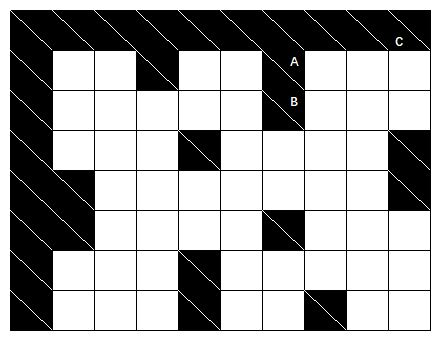
\includegraphics[width=2.2in]{generation1.jpg}
                    \caption[生成1]{生成Kakuro过程1}\label{gen1}
                \end{minipage}
                \begin{minipage}[t]{0.49\linewidth}
                    \centering
                    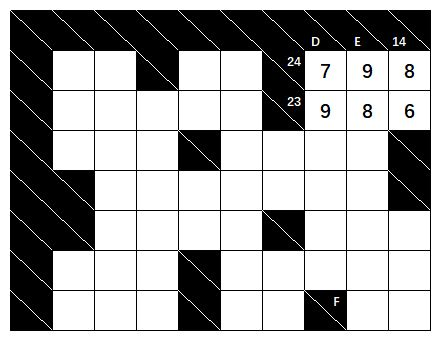
\includegraphics[width=2.2in]{generation2.jpg}
                    \caption[生成2]{生成Kakuro过程2}\label{gen2}
                \end{minipage}
            \end{figure}

            观察数独右上角, $A$和$B$都是长度为3的约束,$C$是长度为2的约束.
            我们知道, 只有一种可能分解的长度为3的约束有3, 4, 23和24.
            我们选择24和23分别作为$A$和$B$和行约束,
            发现分别从两个约束中取值, 和为14的情况只有一种, 就是24中的8加上23中的6,
            于是我们选择14作为$C$的列约束, 此时右上角的6个元素已经被确定(见图\ref{gen2}).

            观察$E$所在列, 与$F$所在行有交叉, 并且已经填入了8和9.
            而$F$约束的长度为2, 当$F$的取值为14, 15, 16或17时都能唯一确定$F$约束下的数字,
            我们选取了16作为$F$的取值.
            再看$D$和$E$的约束, 长度分别为6和7.
            不妨使其组合唯一来防止刚开始生成的时候就有过多的可能性.
            此时$D$约束的可能取值为38和39, $E$约束的可能取值为41和42.
            我们取$D$约束为38, $E$约束为42,
            并在$D$列和$E$列记下每个白格子策略集中的元素(见图\ref{gen3}).

            \begin{figure}[htb]
                \begin{minipage}[t]{0.49\linewidth}
                    \centering
                    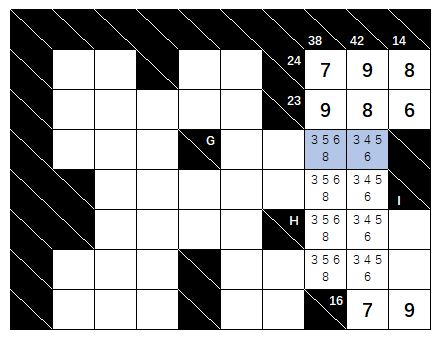
\includegraphics[width=2.2in]{generation3.jpg}
                    \caption[生成3]{生成Kakuro过程3}\label{gen3}
                \end{minipage}
                \begin{minipage}[t]{0.49\linewidth}
                    \centering
                    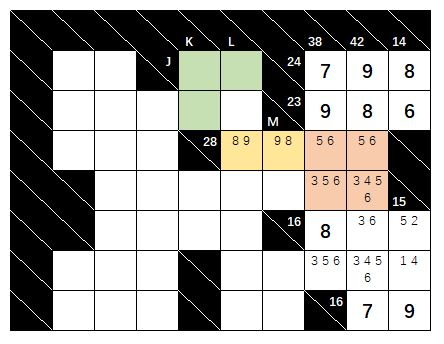
\includegraphics[width=2.2in]{generation4.jpg}
                    \caption[生成4]{生成Kakuro过程4}\label{gen4}
                \end{minipage}
            \end{figure}

            观察$G$的行约束, 如果值为29, 那么可以推出左边的蓝色格子值8,
            右边的蓝色格子值为5, 这样显得太简单了.
            于是我们放宽了$G$的行约束, 取值为28.
            此时, 两个蓝色格子中都不能填入3,
            而且如果右边的蓝色格子填入了4, 那么左边的蓝色格子只能填入8.
            根据这一层推理, 我们要设法使左边的蓝色格子不能填入8,
            这样还能同时缩小右边蓝色格子的策略集.
            观察到行约束$H$右边的两个格子, 如果左边的那个格子不填入8,
            那么这两个格子的和最大仅为11.
            据此, 我们在$H$取比较大的约束, 在$I$取比较小的约束,分别为16和15,
            使得如果$H$右边的第一个格子不填入8, 那么$H$与$I$交叉的那个格子无法取到足够小,
            使得$I$列的和不超出$I$的约束.
            因此, 此时$H$行右边的一个格子的值为8. 更新各格子的策略集(见图\ref{gen4}).

            注意, 虽然16和15在3个数中的和不算大也不算小,
            但是在这种情况下, 它们却共同约束了$H$行左边的格子只能填入8,
            这实在是让人惊叹.

            这时我们发现, 因为上方2个红色格子中只可能是分别填入5和6,
            因此2个黄色格子中只可能分别填入8和9.
            为了确定2个黄色格子的取值, 我们从$J$和$K$这两个长度为2的约束入手.
            如果想让$L$下方的绿色格子取到9, 那么我们需要让$J$取偏大的值, 让$K$取偏小的值,
            类似于之前对$H$和$I$的处理, 取$J$为14, 取$K$为6,
            那么3个绿色格子和2个黄色格子的取值都能确定.
            这时候, 4个红色格子都能取5,6两个值, 为了不让它们导致非唯一解,
            在$M$下方第二个格子我们选择填入6, 即列约束$M$取值为15.
            至于$L$, 随意选了一个组合不过多且满足行内8与9的数37(组合为3种).
            更新各格子的策略集(见图\ref{gen5}).

            \begin{figure}[htb]
                \begin{minipage}[t]{0.49\linewidth}
                    \centering
                    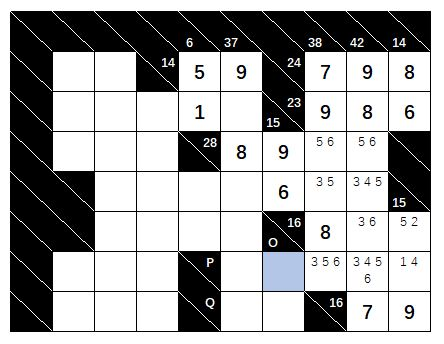
\includegraphics[width=2.2in]{generation5.jpg}
                    \caption[生成5]{生成Kakuro过程5}\label{gen5}
                \end{minipage}
                \begin{minipage}[t]{0.49\linewidth}
                    \centering
                    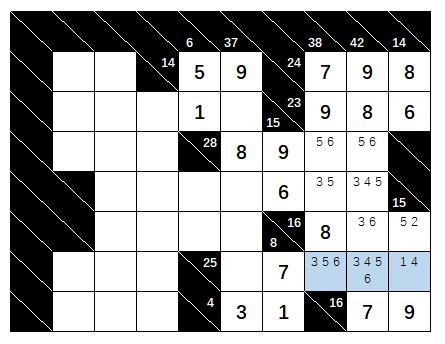
\includegraphics[width=2.2in]{generation6.jpg}
                    \caption[生成6]{生成Kakuro过程6}\label{gen6}
                \end{minipage}
            \end{figure}

            到现在为止, 依旧没有足够的信息来确定右边那一个区域的白格子.
            最后的切入口在中下方$P$, $Q$和$O$三个约束那里.

            经试验, 如果蓝色格子填入5, 那么蓝色格子右边三个的数的和至多达到12,
            并非$6+5+4=15$, 再由于蓝色格子的左边已经不能填入8或者9,
            所以此时5个格子的和不超过24.
            因此我们取定行约束$P=25$, 这样蓝色格子就不能填入5了.
            $P$确定下来之后, 需要确定$O$和$Q$的取值.
            它们的取值需要满足下列要求:
            \begin{itemize}
                \item 如果无视约束$P$, 那么蓝色格子填入5不会引起矛盾.
                \item 在$P$有约束的情况下, 蓝色格子的取值尽可能唯一.
            \end{itemize}
            经过反复斟酌, 我们取了$O=8$, $Q=4$, 此时数独情况如图\ref{gen6}.

            图中三个蓝格子, 取值范围为$\{1,3,4,5,6\}$.
            我们在25-in-5的12种组合中寻找至少包含$\{1,3,4,5,6\}$中三个元素, 且包含7的组合,
            发现了4组, 分别为$\{1,3,5,7,9\},\{1,3,6,7,8\},\{1,4,5,7,8\},\{3,4,5,6,7\}$,
            而若要剔除7和$\{1,3,4,5,6\}$中的三个元素后, 满足不与列中的8和9重复的,
            就只有$\{3,4,5,6,7\}$一种组合了.
            因此, 最右边的蓝格子中只能填入4, 进而顺藤摸瓜, 推出整个右边区域的白格子(见图\ref{gen7}).
            检查一下, 39-in-7的那一列已经填入了3, 6, 8, 9, 依旧是有解的.

             \begin{figure}[htb]
                \begin{minipage}[t]{0.49\linewidth}
                    \centering
                    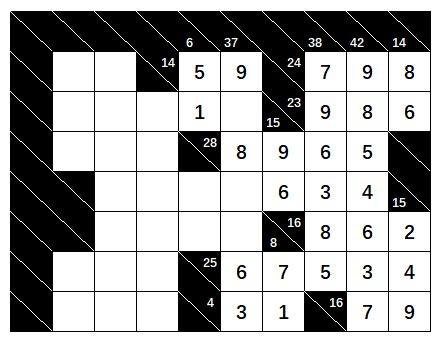
\includegraphics[width=2.2in]{generation7.jpg}
                    \caption[生成7]{生成Kakuro过程7}\label{gen7}
                \end{minipage}
                \begin{minipage}[t]{0.49\linewidth}
                    \centering
                    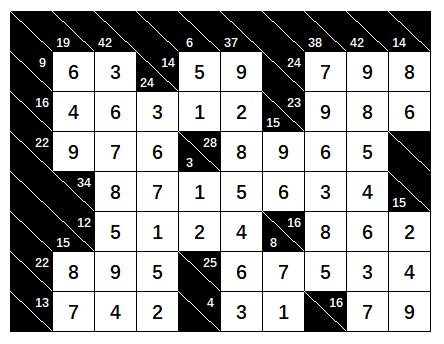
\includegraphics[width=2.2in]{generation8.jpg}
                    \caption[生成8]{生成Kakuro结果}\label{gen8}
                \end{minipage}
            \end{figure}

            至此, 我们已经给出了如何从空数独开始, 从小到大,
            一点一点生成数独的主要方法, 之后的具体生成过程就不再列出了.
            在此给出最后的生成结果(见图\ref{gen8})以及难度评级(见表\ref{tabDfc}).

            除此之外, 我们还生成了一个较简单的数独, 生成结果和难度评级分别能在附录中和前文找到.

    \subsection{蜂巢数独求解}
        蜂巢数独求解和Kakuro求解问题类似, 我们将采用回溯的思想.
        但是此问题和Kakuro问题有所不同, Kakuro问题, 我们采用的深度搜索树的概念比较深刻,
        而蜂巢数独问题十分类似信息学的一个经典问题-八皇后\citep{Baidu_EightQueens},
        其所用的回溯思想更加明显, 因此我们的算法将基于八皇后的回溯思想进行.

        下面许多概念可从之前Kakuro求解算法中类比过来, 这里不再一一赘述.

        \subsubsection{算法概述}
            首先对于第$i$行的元素在该行的策略集中所有可能的策略进行枚举, 判定策略满足约束条件之后,
            转到计算第$i+1$的状态.
            如果$i+1$行的所有策略均不能满足约束, 则回退, 继续枚举第$i$行其它可能的策略.
            这样循环下去, 直到所有的格子都被填充完毕, 算法结束.

        \subsubsection{基本策略集}
            对于蜂巢数独的第$i$行, 记其长度为$l_{i}$, $l_{i}$为确定值.
            定义第$i$行的\textbf{基本策略集} $S_{l_{i}}$:
            所有连续的且元素数目为$l_{i}$的所有排列的集合.
            例如, 当$i=1\ \text{or}\ 9$, $l_{i}=5$时,
            其基本策略集
                \begin{equation*}
                    \begin{split}
                    S_{l_{i}}= S_{5}
                              & = P(1,2,3,4,5)\cup P(2,3,4,5,6)\\
                              & \qquad\cup P(3,4,5,6,7)\cup P(4,5,6,7,8)\cup P(5,6,7,8,9).
                    \end{split}
                \end{equation*}

        \subsubsection{可行性剪枝}
            \subsubsubsection{行内可行性}
                如果在第$i$行有些格子已经由题目给出, 那么我们在枚举$S_{L_{i}}$策略集内排列的时候,
                需要将每种排列与第$i$行题目给出的元素进行比对,
                只有完全匹配的时候, 才能将该排列当作一种策略.
            \subsubsubsection{行间可行性}
                当我们枚举第$i$行策略集的内部排列时, 如果该排列与第$i-1$行在左撇列或者右撇列有数字重复,
                则不满足蜂巢数独的规则, 那么该排列不能当作可行的策略.

                程序中, 我们建立了bool数组Vis\_Left[$s$][$k$](Vis\_Right[$s$][$k$]),
                其中$s$为一个格子所在的左撇列(右撇列)的序号,
                $k$为该格子在行排列中的位数.
                只有两个标记数组均给出false, 才表示第$k$位可行,
                只有一个行排列的每个位数均可行, 此排列才能作为该行的策略.

        \subsubsection{最优化剪枝}
            因为蜂巢数独需要保证数字的连续, 所以如果我们填入的一个数,
            与其所在左撇列(右撇列)一个已经确定的数的差值大于或等于该列的长度,
            那么该左撇列(右撇列)的连续性肯定会被破坏.
            于是此种排列不能作为一种有效的策略, 应该舍去.

            \begin{figure}[htb]
                \centering
                \includegraphics[scale = 0.5]{example5.bmp}
                \caption[例5]{蜂巢数独最优化剪枝的例子}\label{exm5}
            \end{figure}
            以题干为例子(见图\vref*{exm5}), 当搜索到第五行时(实际上前四行已经填满但图中未标识),
            第五行第一个格子可以填写\{1,3,4,6,7,8,9\},但是填写$7,8\ \text{or}\ 9$时,
            有\[|9-2|\geq|8-2|\geq|7-2|\geq5,\]
            因此, 首位数字是7, 8或9的排列可以被剪枝.

        \subsubsection{算法检验与效果测试}
            因为采用了大量的剪枝, 所以程序有很好的效率.
            运行样例的两组数据, 得到以下结果:
            \begin{table}
                \begin{center}
                    \caption[蜂巢数独结果]{样例蜂巢数独程序运行结果}
                    \begin{tabular}{ccc}
                        \Xhline{1.2pt}
                        组号  &   递归次数    &   运行时间\\
                        \hline
                        第一组 &   39  &   109ms\\
                        第二组 &   52  &    78ms\\
                        \Xhline{1.2pt}
                    \end{tabular}
                \end{center}
            \end{table}
            求解时间在0.1秒左右, 搜索次数的数量级也只在几十次.
            可见, 本算法是一种高效的解决方案.
            实现算法将附\vpageref*[][]{prgBee},
            程序运行结果截图将附\vpageref*[][]{resBee}.

%===============CONCLUSION===============
\section{结论}
    \paragraph{优点:}
        \begin{itemize}
            \item
                本文建立的Kakuro数独和蜂巢数独求解模型, 对任务1和任务4实现了完美的解决,
                在所搜集的到不同难度的数独中, Kakuro数独都能在1秒内实现求解,
                而蜂巢数独的求解时间甚至达到了0.1秒以内.
            \item
                本文建立的难度分级系统, 基于深度优先搜索树和归谬法剪枝次数,
                实现了对不同难度的准确分级,
                且分级结果是稳定的, 不受搜索策略枚举顺序的影响.
            \item
                本文使用演绎法生成Kakuro, 可以保证生成的Kakuro具有唯一解,
                并且能预先指定生成Kakuro的难度.
        \end{itemize}
    \paragraph{需要改进之处}
        \begin{itemize}
            \item
                本文的难度分级系统, 最后具体的分类界线画的比较随意,
                没有进行过大量数据的测试和修正, 导致可能最后会被分进简单难度的数独很少.
            \item
                本文中的演绎法生成Kakuro, 生成效率比较低下, 生成困难的数独可能要花好几个小时的时间.
                而且生成难度较大数独的时候, 有时也需要碰运气, 如果添加了许多约束但最后发现了矛盾,
                就会浪费很多时间.
        \end{itemize}
    \newpage

%===============REFERENCE===============
\section*{参考文献}
    \bibliography{Kakuro}
    \bibliographystyle{unsrt}

    \newpage

%===============APPENDICES===============
\section*{附录}
    \addcontentsline{toc}{section}{\numberline{} 附录}
    \subsection*{程序运行结果}
        \begin{figure}[htb]
            \centering
            \includegraphics{result1.bmp}
            \caption[结果1]{样例Kakuro的求解结果}\label{resKak}
        \end{figure}
        \begin{figure}[htb]
            \centering
            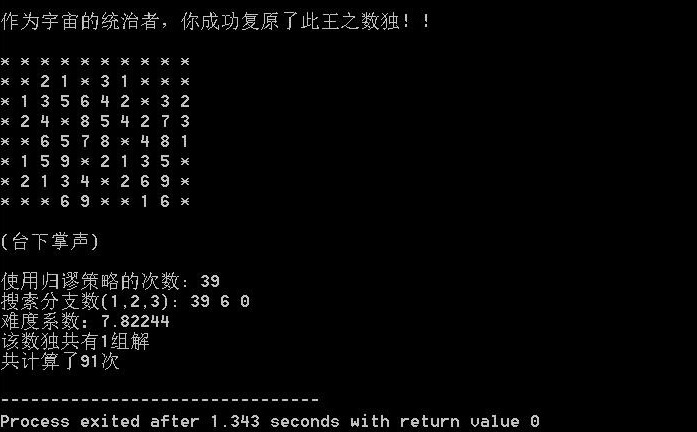
\includegraphics[scale = 0.5]{result3-1.jpg}
            \caption[结果3-1]{样例Kakuro的难度分析结果}\label{resDfc}
        \end{figure}
        \begin{figure}[htb]
            \centering
            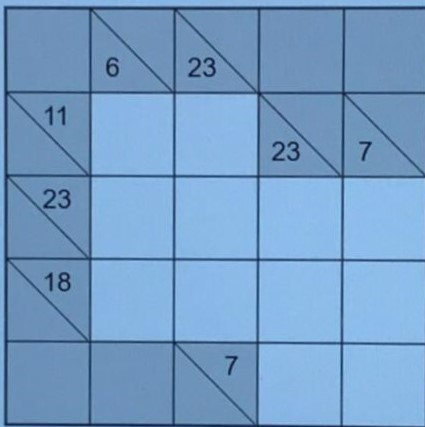
\includegraphics[scale = 0.5]{result3-2-1.jpg}
            \caption[数独3-2]{第一个简单难度Kakuro}
        \end{figure}
        \begin{figure}[htb]
            \centering
            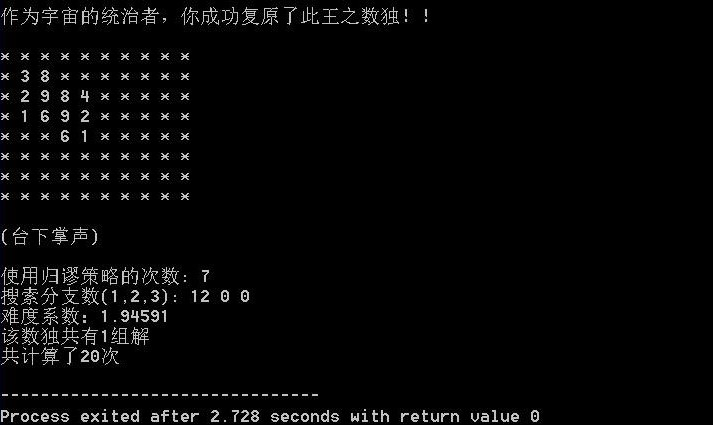
\includegraphics[scale = 0.5]{result3-2-2.jpg}
            \caption[结果3-2]{第一个简单难度Kakuro的难度分析结果}
        \end{figure}
        \begin{figure}[htb]
            \centering
            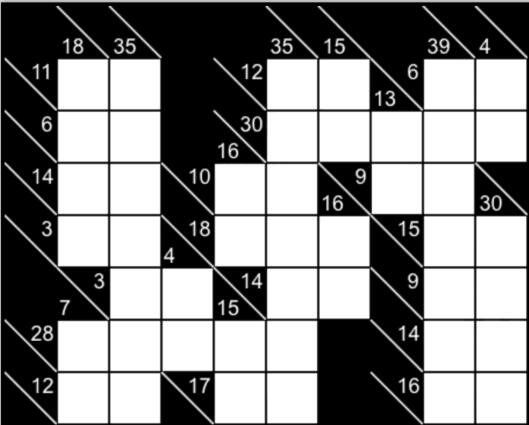
\includegraphics[scale = 0.5]{result3-3-1.jpg}
            \caption[数独3-3]{第二个简单难度Kakuro}
        \end{figure}
        \begin{figure}[htb]
            \centering
            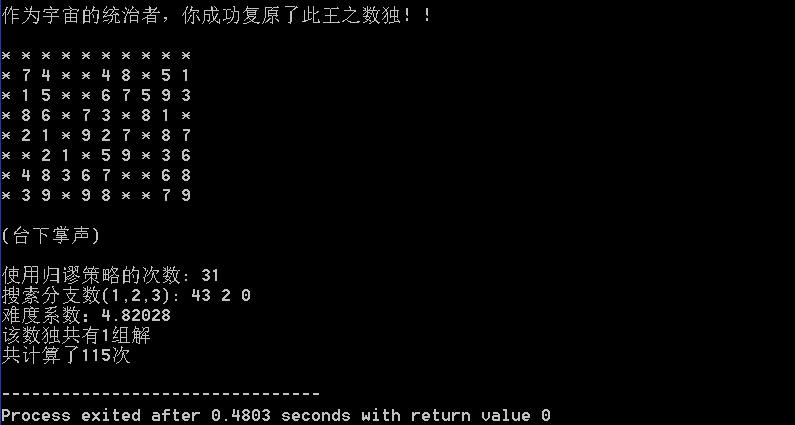
\includegraphics[scale = 0.5]{result3-3-2.jpg}
            \caption[结果3-3]{第二个简单难度Kakuro的难度分析结果}
        \end{figure}
        \begin{figure}[htb]
            \centering
            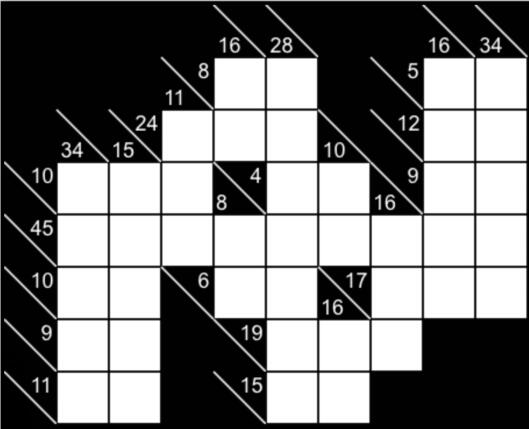
\includegraphics[scale = 0.5]{result3-4-1.jpg}
            \caption[数独3-4]{中等难度Kakuro}
        \end{figure}
        \begin{figure}[htb]
            \centering
            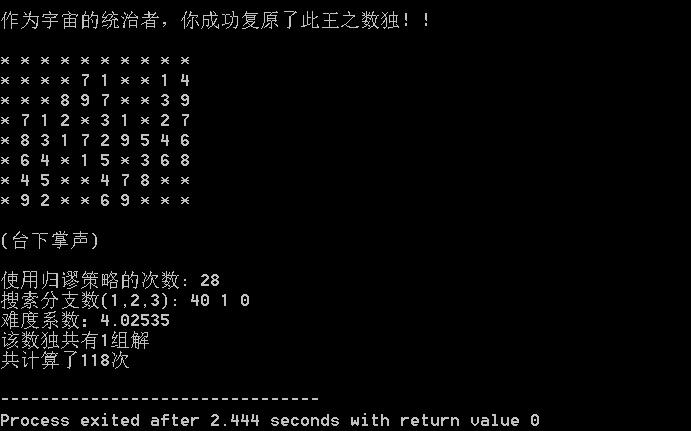
\includegraphics[scale = 0.6]{result3-4-2.jpg}
            \caption[结果3-4]{中等难度Kakuro的难度分析结果}
        \end{figure}
        \begin{figure}[htb]
            \centering
            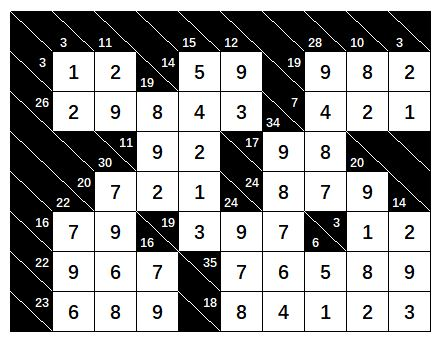
\includegraphics[scale = 0.6]{result3-5-1.jpg}
            \caption[数独3-5]{自己生成较简单的Kakuro}
        \end{figure}
        \begin{figure}[htb]
            \centering
            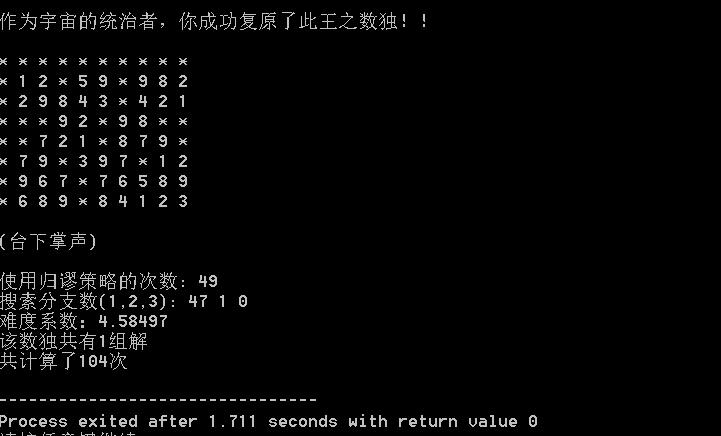
\includegraphics[scale = 0.6]{result3-5-2.jpg}
            \caption[结果3-5]{自己生成较简单的Kakuro的难度分析结果}
        \end{figure}
        \begin{figure}[htb]
            \centering
            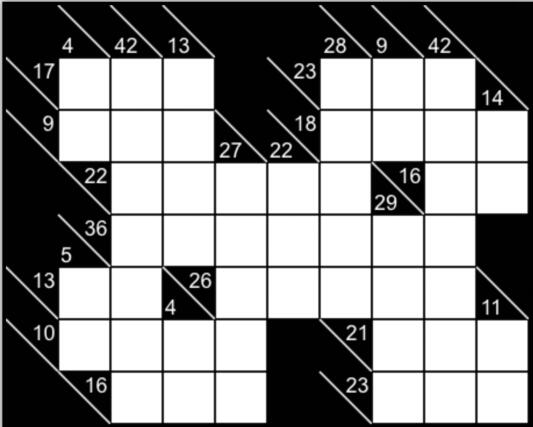
\includegraphics[scale = 0.5]{result3-6-1.jpg}
            \caption[数独3-6]{第一个困难难度Kakuro}
        \end{figure}
        \begin{figure}[htb]
            \centering
            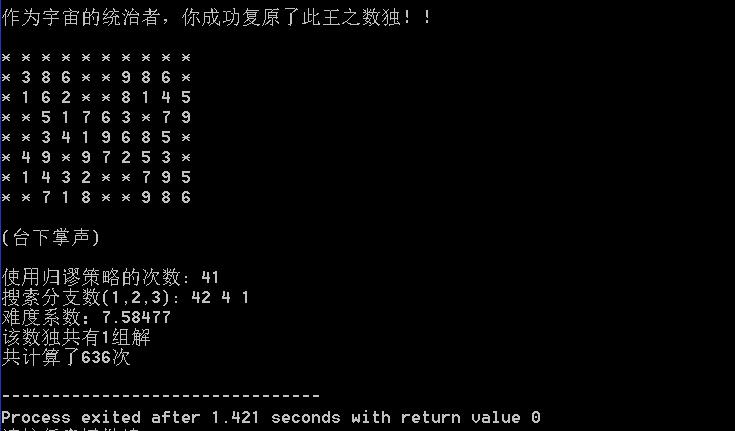
\includegraphics[scale = 0.6]{result3-6-2.jpg}
            \caption[结果3-6]{第一个困难难度Kakuro的难度分析结果}
        \end{figure}
        \begin{figure}[htb]
            \centering
            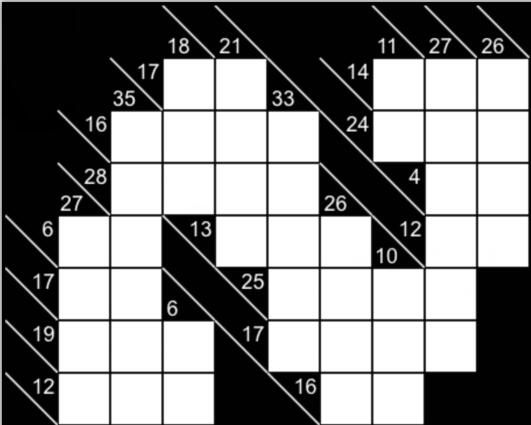
\includegraphics[scale = 0.5]{result3-7-1.jpg}
            \caption[数独3-7]{第二个困难难度Kakuro}
        \end{figure}
        \begin{figure}[htb]
            \centering
            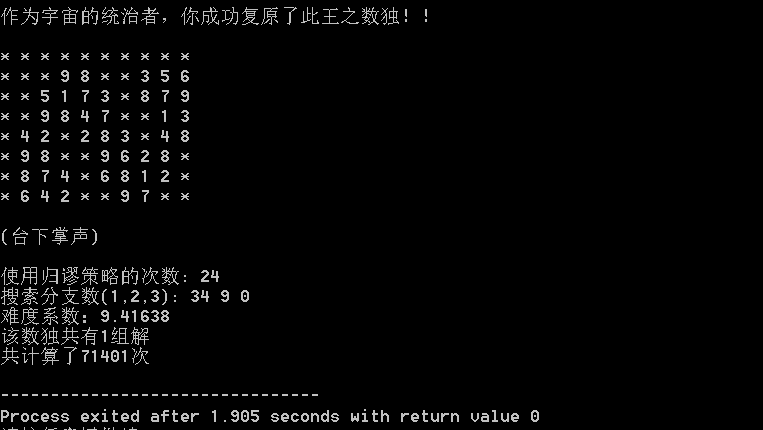
\includegraphics[scale = 0.4]{result3-7-2.jpg}
            \caption[结果3-7]{第二个困难难度Kakuro的难度分析结果}
        \end{figure}
        \begin{figure}[htb]
            \centering
            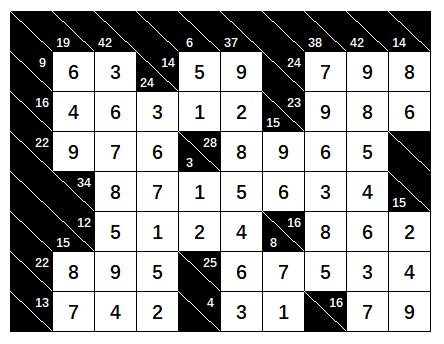
\includegraphics[scale = 0.5]{generation8.jpg}
            \caption[数独3-8]{自己生成地狱难度Kakuro}
        \end{figure}
        \begin{figure}[htb]
            \centering
            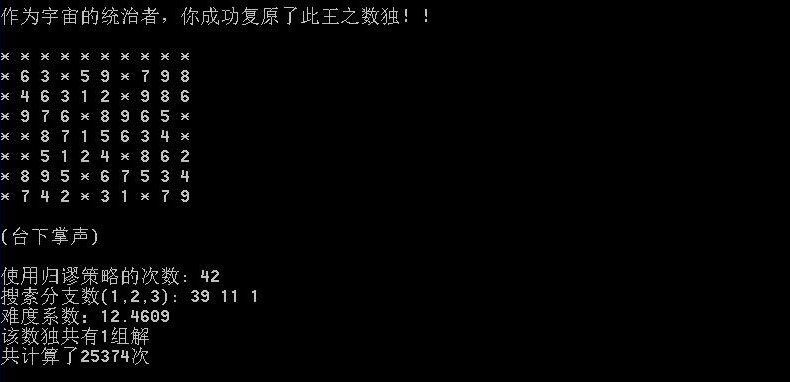
\includegraphics[scale = 0.4]{result3-8-2.jpg}
            \caption[结果3-8]{自己生成地狱难度Kakuro的难度分析结果}
        \end{figure}
        \begin{figure}[htb]
            \centering
            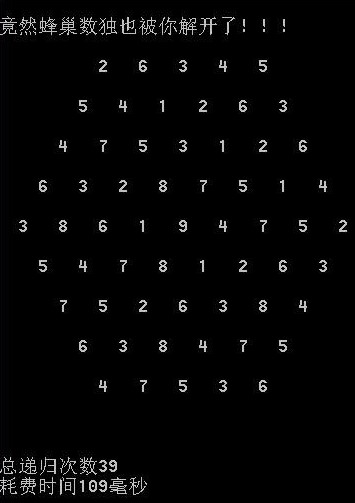
\includegraphics[scale = 0.5]{result4-1.jpg}
            \caption[结果4-1]{蜂巢数独样例1的求解结果}\label{resBee}
        \end{figure}
        \begin{figure}[htb]
            \centering
            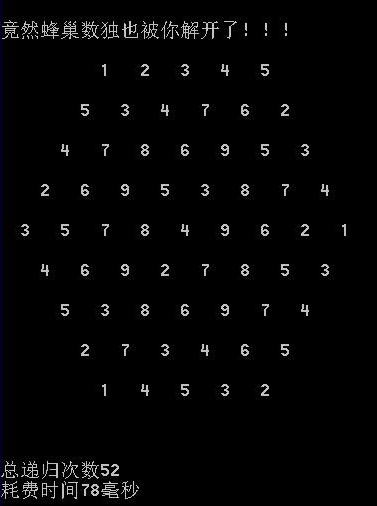
\includegraphics[scale = 0.5]{result4-2.jpg}
            \caption[结果4-2]{蜂巢数独样例2的求解结果}
        \end{figure}


\end{document}
